\section{Task 1: One file}

\subsection{Task 1a: Counting with threads}

\textbf{Implementation} (\texttt{Task1a.java}). With $N$ threads the file of $S$ bytes is divided
into $N$ byte ranges $[\,S\cdot i/N,\; S\cdot(i+1)/N\,)$. Every thread opens its own
\texttt{RandomAccessFile}, seeks to the start of its range and reads it in 1\,MiB blocks into its
own buffer, parsing the bytes as they come (\texttt{LineParser}: digits are accumulated, a
\texttt{-} sets the sign, \texttt{\textbackslash n} ends the number) and counting into its own
\texttt{Counts} object. The main thread joins the threads and adds their counts. No thread reads
the whole file.

A byte range usually starts and ends in the middle of a line, so one rule decides who owns each
line: \emph{a line belongs to the range in which its first byte lies.} Two consequences follow:
\begin{itemize}
\item a thread first looks at the byte just before its range; if it is not \texttt{\textbackslash n},
the range starts inside a line that the previous thread owns, so the thread skips bytes up to and
including the next \texttt{\textbackslash n};
\item a thread keeps reading after the end of its range until it finishes the last line it has
started, and it stops as soon as the next line would start at or after its end.
\end{itemize}
Because every line has exactly one first byte, and that byte is in exactly one range, every line
is counted by exactly one thread. I checked the rule on a small file with every thread count from
1 to 64 (more threads than lines included), with \texttt{\textbackslash r\textbackslash n} line
ends and without a final newline, and on the real file: every run gave exactly 50\,000\,000 numbers
and the expected totals.

\begin{figure}[H]
\centering
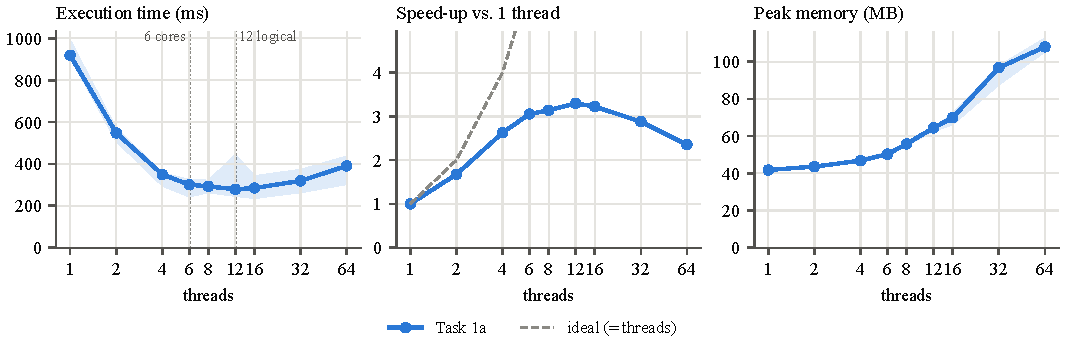
\includegraphics[width=\textwidth]{figures/task1a.pdf}
\caption{Task 1a: time, speed-up and peak memory against the number of threads (median of 5 runs;
the band shows the fastest and slowest run; dotted lines: 6 physical cores, 12 logical processors)}
\label{fig:1a}
\end{figure}

\begin{table}[H]
\centering\small
\begin{tabular}{rrrrr}
\toprule
Threads & Median time (ms) & Min--max (ms) & Speed-up & Peak memory (MB) \\
\midrule
1 & 919 & 908--996 & 1.00 & 42 \\
2 & 548 & 507--572 & 1.68 & 44 \\
4 & 350 & 294--359 & 2.63 & 47 \\
6 & 301 & 242--326 & 3.05 & 50 \\
8 & 293 & 262--323 & 3.14 & 56 \\
12 & 279 & 245--446 & 3.30 & 64 \\
16 & 285 & 235--344 & 3.22 & 70 \\
32 & 319 & 262--375 & 2.88 & 97 \\
64 & 391 & 301--438 & 2.35 & 108 \\
\bottomrule
\end{tabular}

\caption{Task 1a results}
\label{tab:1a}
\end{table}
